\documentclass{article}
\usepackage[utf8]{inputenc}
\usepackage[T1]{fontenc}
\usepackage{geometry}
\geometry{left=2.5cm,right=2.5cm,top=2.5cm,bottom=2.5cm}
\usepackage{graphicx}
\usepackage{float}
\usepackage{amsmath}
\usepackage{amssymb}
\usepackage{cite}
\usepackage{hyperref}
\usepackage{listings}
\usepackage{xcolor}
\usepackage{booktabs}
\usepackage{caption}
\usepackage{subcaption}
\usepackage{algorithm}
\usepackage{algpseudocode}
\usepackage{tikz}
\usepackage{pgfplots}
\pgfplotsset{compat=1.16}
\usetikzlibrary{shapes,arrows,positioning,fit,backgrounds,matrix,calc}

\definecolor{bluebox}{RGB}{230,240,255}
\definecolor{greenbox}{RGB}{230,255,230}
\definecolor{redbox}{RGB}{255,230,230}
\definecolor{orangebox}{RGB}{255,245,220}

\lstset{
    basicstyle=\ttfamily\small,
    breaklines=true,
    frame=single,
    backgroundcolor=\color{gray!10},
    keywordstyle=\color{blue},
    commentstyle=\color{green!60!black},
    stringstyle=\color{red}
}

\title{A GDPR Compliance Warning Framework Based on Android Permission Auditing: Design, Implementation and Adversarial Evaluation}
\author{Zhiheng Zhang}
\date{July 2026}

\begin{document}

\maketitle
\newpage
\tableofcontents
\newpage

% ==================== Chapter 1: Introduction (Revision 02) ====================
\newpage
\begin{abstract}
Mobile applications routinely access location, microphone, and contact data, yet platform permission interfaces provide limited support for interpreting whether repeated access is proportionate to a declared purpose. This thesis presents and evaluates a prototype GDPR compliance-warning application that translates permission-access counts into explainable risk findings. The implemented React Native/TypeScript prototype contains a modular compliance engine, explicit rule metadata for three sensitive permission categories, a deterministic threshold calculation, local finding persistence, a violation simulator, and an Android user interface for running and reviewing audits.

Evaluation was performed at both the logical and packaged-application layers. An independent-oracle Monte Carlo test and a boundary-stratified test produced 7,000 zero-error observations for the implemented daily-count rule, with a descriptive 95\% Wilson accuracy lower bound of 99.945\%. A release-APK endurance sequence added 1,500 zero-error integration observations, completed without a captured crash or application-not-responding event, and recorded a peak proportional set size of 115.16~MB. These results validate implementation consistency within the specified rule domain.

A second adversarial campaign exposed limits that conventional accuracy did not reveal. Short-term burst and cross-window split attacks each bypassed the detector in all tested scenarios; all 40,000 invalid time windows were accepted; and 83.776\% of 250,000 combined malformed inputs were silently classified as normal. The study therefore distinguishes rule correctness from threat-model completeness. It concludes that the prototype is a reproducible compliance-warning demonstrator, while production deployment requires fail-closed runtime validation, multi-scale temporal features, privileged or system-mediated Android data acquisition, physical-device endurance testing, and legal review of the warning criteria.
\end{abstract}

\section{Introduction}

\subsection{Background and Motivation}

The General Data Protection Regulation (GDPR) requires personal data to be processed lawfully, transparently, and in a manner limited to what is necessary for the stated purpose. On Android, runtime permission controls make access decisions visible to users, but a grant or denial does not by itself explain whether the frequency of subsequent access is proportionate. A navigation application and a calculator may both request location permission, yet identical access counts can carry very different contextual meanings. Permission frequency is therefore a useful warning signal, but it is not, on its own, a legal determination.

This thesis investigates whether a small, explainable rule engine can turn structured permission-audit observations into reproducible compliance warnings. The work focuses on three sensitive categories represented in the prototype: LOCATION, MICROPHONE, and CONTACTS. For each category, the engine records a baseline, a deviation multiplier, a GDPR mapping, and a plain-language rationale. An observation becomes active when its access count strictly exceeds the calculated threshold. The approach favours transparency: every finding exposes the rule, threshold, excess count, risk level, and regulatory rationale that produced it.

The research is motivated by a practical gap between platform transparency and compliance interpretation. Native privacy dashboards provide useful histories, but users must still interpret whether a pattern is excessive, whether an abnormal record is trustworthy, and whether repeated notifications deserve attention. Conversely, opaque anomaly models may produce a score without an auditable reason. A deterministic prototype provides a controlled setting in which the relationship between an observation and a warning can be examined directly.

\subsection{Problem Statement}

The central problem is not simply to maximise classification accuracy. It is to establish what a warning means, which inputs it trusts, and which behaviours its model can observe. Three related challenges follow.

\begin{enumerate}
    \item \textbf{Explainable operationalisation.} GDPR principles are contextual legal standards. A software prototype must not claim that a frequency threshold proves illegality. It can, however, identify a pattern that warrants review and show the rule used to reach that conclusion.
    \item \textbf{Reliable implementation.} The same structured observation must produce the same result across random, boundary, and repeated APK execution. An external test oracle is required to avoid validating the implementation against itself.
    \item \textbf{Adversarial completeness.} High accuracy over valid count inputs does not establish resistance to burst timing, cross-window splitting, forged timestamps, type confusion, or malformed permission identifiers. These dimensions require separate oracles and metrics.
\end{enumerate}

This distinction is especially important for a compliance tool. A false assurance can be more harmful than an explicit rejection because it may enter an audit trail as an apparently valid normal result. The framework is therefore evaluated for both incorrect classifications and unsafe acceptance.

\subsection{Research Questions}

The study addresses the following research questions:

\begin{enumerate}
    \item Can a modular, explainable engine implement permission-specific aggregate-count warning rules consistently across random and boundary inputs?
    \item Does the packaged Android application preserve this correctness and remain operational during accelerated repeated execution?
    \item Which previously unmodelled temporal and runtime-input attacks can bypass or destabilise the current prototype?
    \item What implementation and validation work is required before the prototype can support broader operational claims?
\end{enumerate}

\subsection{Objectives and Contributions}

The first objective is to produce an auditable prototype rather than an opaque classifier. The TypeScript \texttt{GDPRComplianceEngine} implements the \texttt{IComplianceEngine} interface and uses an explicit rule table. The current thresholds are calculated as the ceiling of a fixed baseline multiplied by 1.5: 36 for LOCATION, 12 for MICROPHONE, and 6 for CONTACTS. Findings retain the permission, package identifier, threshold, excess count, risk level, detection time, GDPR article mapping, and rationale.

The second objective is to connect this logic to a usable Android demonstrator. The React Native application provides experiment, privacy, history, scoring, and settings views. Synthetic configurations are converted into audit observations, evaluated locally, and persisted with AsyncStorage. The repository also contains a native-bridge boundary for future Android acquisition and scheduling functions. Those optional native functions are not treated as validated production capabilities in this thesis.

The third objective is methodological. The evaluation separates independent-oracle logical tests, release-APK integration tests, and adversarial tests. The contribution is not merely a large execution count, but an evidence structure that prevents a correct implementation of a narrow rule from being presented as complete attack detection.

The principal contributions are:

\begin{itemize}
    \item an explainable and modular compliance-warning rule engine for three sensitive permission categories;
    \item a locally operated Android demonstrator with reproducible simulation and finding persistence;
    \item a progressive validation protocol combining independent random sampling, threshold-boundary stratification, APK endurance, and Android event fuzzing;
    \item a second adversarial protocol that quantifies temporal bypass, invalid-window acceptance, runtime type confusion, permission-key mutation, and combined malformed inputs; and
    \item an evidence-based set of priorities for fail-closed validation, temporal modelling, UI regression, and future native Android integration.
\end{itemize}

\subsection{Scope}

The implemented and evaluated scope is deliberately bounded. The engine evaluates structured observations supplied by the simulator or application workflow. The study does not demonstrate unrestricted collection of other applications' permission history on a stock physical device, does not establish 24- or 72-hour WorkManager reliability, and does not measure battery drain. It also does not determine GDPR liability. The output is a warning that supports review, not a binding legal conclusion.

This boundary improves rather than weakens the research claim. It permits the tested logic, APK behaviour, observed vulnerabilities, and untested production assumptions to be stated separately. The resulting account is reproducible and avoids attributing native Android capabilities to code paths that were not exercised.

\subsection{Thesis Structure}

Chapter 2 reviews GDPR principles, privacy-warning design, Android auditing constraints, and security-testing methods. Chapter 3 derives the requirements and presents the architecture of the implemented prototype, including explicit trust boundaries. Chapter 4 explains the TypeScript rule engine, simulator, local repository, bridge boundary, and user-interface integration. Chapter 5 reports both iterative test campaigns and their statistical interpretation. Chapter 6 discusses trade-offs, validity, legal and platform limitations, and repair priorities. Chapter 7 answers the research questions, summarises the supported contributions, and defines the work required for a production-oriented system.

% ==================== Chapter 2: Literature Review (Revision 03) ====================
\newpage
\section{Literature Review and State of the Art}

\subsection{From GDPR Principles to Technical Warning Signals}

Article 5 of the GDPR establishes lawfulness, fairness, transparency, purpose limitation, data minimisation, accuracy, storage limitation, integrity, confidentiality, and accountability \cite{1}. Article 5(1)(c) requires personal data to be adequate, relevant, and limited to what is necessary. Article 25 further requires data protection by design and by default. These provisions motivate technical mechanisms that make data processing observable, but they do not define a universal numeric limit for permission access.

This distinction determines the role of the proposed framework. A high access count may be legitimate for navigation and disproportionate for a calculator. A threshold crossing is therefore an auditable warning signal rather than proof of a GDPR infringement. Purpose, lawful basis, user expectations, foreground context, data destination, and safeguards remain relevant to any legal assessment. The prototype operationalises only one observable component: whether a structured permission count exceeds an explicit, permission-specific rule.

Article 7 concerns the conditions for consent and withdrawal, while Article 9 imposes additional conditions on special-category data. Location, microphone, and contact information are not automatically special-category data in every context, although they may reveal health, biometric, religious, political, or other protected information. The engine's GDPR mappings are consequently explanatory prompts. They identify provisions that may require review and do not replace a controller's legal analysis.

\subsection{Transparency, Cognitive Load, and Warning Design}

Privacy notices impose a substantial verification burden on users. Long policies and frequent prompts encourage heuristic decision-making, while repeated low-value warnings can create habituation and privacy fatigue \cite{12,13,27}. Cognitive Load Theory suggests that information should be structured so that users can identify the reason for an intervention without processing unnecessary detail \cite{27}. Trust in automation likewise depends on calibrated rather than unconditional reliance \cite{34}.

These findings support three interface principles used by the prototype. First, a finding should expose its threshold, observed count, risk level, and rationale. Second, unchanged findings should not repeatedly demand attention. Third, severity should be interpretable and should not imply legal certainty. The local repository therefore records whether a finding changed and whether notification would be justified by a state transition or risk escalation.

The evaluation in this thesis does not include a user study. Claims that the interface reduces cognitive load or improves privacy decisions remain design hypotheses. A longitudinal study using behavioural measures and instruments such as NASA-TLX would be required to validate those effects \cite{6}.

\subsection{Android Permission Transparency and Acquisition Constraints}

Android has progressively expanded runtime permission controls and system privacy interfaces. The Privacy Dashboard introduced a system-managed history for selected sensitive permissions, providing users with temporal visibility. However, access to app-operation history by a third-party application is constrained by Android version, privileges, attribution, and vendor implementation. Public presence of an \texttt{AppOpsManager} method does not imply that an ordinary sandboxed application can retrieve unrestricted histories for every other package.

This constraint divides a complete system into two parts. The decision layer can be implemented and tested using structured \texttt{PermissionAudit} observations. The acquisition layer requires an authorised source, such as system integration, device-owner deployment, user-mediated export, or another platform-supported mechanism. The current repository validates the former and exposes a React Native native-module boundary for the latter; it does not claim that unrestricted cross-application acquisition was demonstrated on a stock physical device.

Static-analysis systems such as FlowDroid and dynamic taint-tracking systems address different questions. They seek code paths or data flows from sensitive sources to sinks, often at greater deployment and computational cost. VPN-based monitoring observes network traffic but cannot directly observe local permission use and introduces its own trust boundary. Native dashboards are low-overhead and authoritative but do not provide the custom rule evaluation developed here. The proposed prototype therefore occupies a narrower position: explainable evaluation of supplied permission-frequency observations.

\subsection{Rule-Based and Statistical Detection}

Rule-based systems are attractive for compliance warnings because their outputs can be traced to an explicit condition. They also expose their limitations. A fixed threshold ignores temporal concentration and application purpose, while a learned anomaly model can be difficult to explain and may drift as behaviour changes. Hybrid systems may combine population priors, per-user history, and contextual features, but those additions require empirical data and independent validation.

The implemented prototype uses fixed expert-configured baselines multiplied by 1.5. It does not compute a rolling mean, standard deviation, or three-sigma threshold, and it does not contain a validated population study of the top 50 applications. Those mechanisms remain possible extensions, not evaluated features. This factual boundary is essential because a claimed adaptive model cannot be supported by experiments that exercise a deterministic fixed rule.

The current rule is intentionally simple:

\begin{equation}
T_p=\left\lceil 1.5B_p \right\rceil,\qquad
A(x,p)=\mathbb{I}[x>T_p],
\end{equation}

where $B_p$ is the configured baseline for permission $p$, $T_p$ is the threshold, $x$ is the supplied access count, and $A$ is the active-warning decision. Simplicity makes exhaustive boundary reasoning possible, but it also makes temporal bypass predictable unless time-derived features are added.

\subsection{Randomised, Boundary, and Adversarial Validation}

Randomised testing explores a larger input space than a small hand-written suite. Its value depends on the oracle and distribution. If the expected result is produced by the same helper used by the system under test, perfect agreement may merely demonstrate shared logic. The evaluation therefore introduces an external oracle for the main Monte Carlo round and separately concentrates samples at $T_p-2$ through $T_p+2$.

Boundary testing is necessary because random uniform inputs may rarely land close to a threshold. Adversarial testing asks a different question: what happens when assumptions are violated? Fuzzing permission keys, numeric types, and time windows tests the runtime trust boundary; burst and split-window samples test omissions in the decision model. These cases cannot all be placed in a conventional confusion matrix, because they use different threat definitions and expected failure policies.

Confidence intervals are also required for honest interpretation. An observed accuracy of 100\% is a point estimate. Wilson intervals and the rule of three express the uncertainty remaining after zero observed errors. Repeated deterministic mutations are useful for stress and reproducibility, but repetitions of the same mutation class should not be described as independent population samples.

\subsection{Research Gap}

Prior approaches typically emphasise one of four goals: platform transparency, static disclosure analysis, data-flow detection, or user notification. The research gap addressed here is a reproducible connection between an explainable permission-frequency rule, a usable Android demonstrator, and an evaluation that explicitly separates correctness from adversarial coverage.

The contribution is accordingly methodological as well as technical. The prototype demonstrates how a compliance-warning decision can be exposed and tested. The negative adversarial results demonstrate why a narrow rule must not be generalised into a claim of complete GDPR compliance detection. Chapters 3 and 4 translate this position into explicit architecture and implementation boundaries, and Chapter 5 evaluates both the supported rule and its uncovered attack surface.

% ==================== Chapter 3: Requirements and Architecture (Revision 04) ====================
\newpage
\section{System Requirements and Overall Design}

\subsection{System Boundary}

The system is a local compliance-warning demonstrator. Its validated input is a structured \texttt{PermissionAudit} containing a package name, one of three supported permission categories, an access count, and an audit-window start and end. Its validated output is an explainable \texttt{ComplianceFinding}. The framework does not intercept calls, block data transfer, determine legal liability, or prove that consent withdrawal has been enforced by another application.

The Android application is implemented with React Native, Expo, and TypeScript. It contains an optional native-module boundary named \texttt{PrivacyInspector}, but the evaluated build does not establish unrestricted acquisition of other applications' AppOps history. Acquisition and decision are therefore separate trust domains:

\begin{itemize}
    \item the \textbf{acquisition domain} is responsible for producing authentic, well-formed observations under an Android-supported authority model;
    \item the \textbf{decision domain} evaluates those observations using transparent rules; and
    \item the \textbf{presentation domain} stores and displays findings without upgrading a warning into a legal conclusion.
\end{itemize}

\subsection{Functional Requirements}

The implemented prototype must:

\begin{enumerate}
    \item evaluate LOCATION, MICROPHONE, and CONTACTS observations through a common engine interface;
    \item expose the threshold, excess count, risk level, GDPR mapping, rationale, and detection time;
    \item generate reproducible benign and violating simulation cases;
    \item persist the latest finding for each package-permission pair locally;
    \item identify whether a finding changed or escalated;
    \item display experiment and privacy results in the Android application; and
    \item permit release-build testing through adb-driven interaction and evidence capture.
\end{enumerate}

Security requirements derived from the adversarial model are stricter than the initial implementation. Permission values must belong to an explicit whitelist. Counts must be finite, non-negative integers. Window timestamps must be finite integers with a valid ordering and bounded duration. Invalid input must produce a structured rejection and an audit record. These requirements are included in the final architecture even though Chapter 5 shows that the current engine does not yet satisfy them.

\subsection{Non-Functional Requirements}

The principal non-functional requirements are explainability, reproducibility, local operation, and bounded resource use. A fixed seed must reproduce logical test sequences. Findings must be understandable without inspecting source code. Personal audit data should remain on the device unless the user deliberately exports it. The release application should remain responsive and below the provisional 150~MB PSS target during accelerated evaluation.

Battery consumption, multi-day scheduling, and manufacturer-specific background behaviour are not accepted as satisfied requirements because they were not measured. They are validation requirements for a future native acquisition layer.

\subsection{Architecture}

The architecture contains five cooperating components.

\begin{enumerate}
    \item \textbf{Compliance engine.} \texttt{GDPRComplianceEngine} implements \texttt{IComplianceEngine} and evaluates one structured audit at a time.
    \item \textbf{Rule configuration.} \texttt{GDPR\_RULES} stores the baseline, deviation multiplier, GDPR mapping, and rationale for each supported permission.
    \item \textbf{Simulation and evaluation.} \texttt{ViolationSimulator} generates configurations and converts them to audits. Evaluation code records confusion-matrix outcomes.
    \item \textbf{Finding repository.} \texttt{ViolationRepository} uses AsyncStorage and determines whether a finding is new, changed, or escalated.
    \item \textbf{Application and bridge boundary.} React Native screens invoke the TypeScript services. \texttt{PrivacyBridge} optionally delegates acquisition, scheduling, and dispatch functions to a native \texttt{PrivacyInspector} module when one is present.
\end{enumerate}

\begin{figure}[H]
\centering
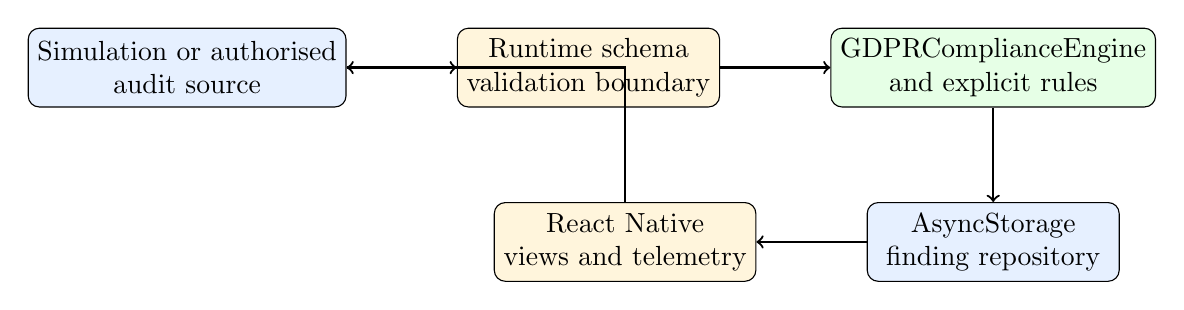
\begin{tikzpicture}[
node distance=1.2cm and 1.4cm,
box/.style={draw, rounded corners, align=center, minimum width=3.2cm, minimum height=1cm},
arrow/.style={->, thick}
]
\node[box, fill=bluebox] (source) {Simulation or authorised\\audit source};
\node[box, fill=orangebox, right=of source] (validation) {Runtime schema\\validation boundary};
\node[box, fill=greenbox, right=of validation] (engine) {GDPRComplianceEngine\\and explicit rules};
\node[box, fill=bluebox, below=of engine] (repo) {AsyncStorage\\finding repository};
\node[box, fill=orangebox, left=of repo] (ui) {React Native\\views and telemetry};
\draw[arrow] (source) -- (validation);
\draw[arrow] (validation) -- (engine);
\draw[arrow] (engine) -- (repo);
\draw[arrow] (repo) -- (ui);
\draw[arrow] (ui) |- (source);
\end{tikzpicture}
\caption{Prototype architecture and the required input-validation boundary}
\label{fig:final-architecture}
\end{figure}

The validation boundary is shown explicitly because it is the highest-priority missing control identified by testing. Its architectural placement ensures that no malformed value reaches threshold lookup or arithmetic.

\subsection{Decision Model}

For each permission $p$, the engine calculates

\begin{equation}
T_p=\max(1,\lceil B_pM_p\rceil),
\end{equation}

where $B_p$ is the configured baseline and $M_p=1.5$. The implemented baselines are 24, 8, and 4, yielding thresholds of 36, 12, and 6. The excess and ratio are

\begin{equation}
E=\max(0,x-T_p),\qquad R=E/T_p.
\end{equation}

A finding is active when $E>0$. Active findings are mapped to MEDIUM, HIGH, or CRITICAL according to the excess ratio; inactive findings are LOW. These severity labels prioritise review and do not state the severity of a legally adjudicated GDPR violation.

\subsection{Temporal Model and Known Coverage Gap}

The input structure contains trigger times and window fields, but the current decision uses only the aggregate count. Consequently, uniform and burst distributions with the same count receive the same verdict, and adjacent windows do not share cumulative state. The final design therefore specifies a later temporal layer containing peak rate, minute/hour/day windows, and decaying cross-window state. This layer is a repair requirement, not an implemented result.

\subsection{Validation Architecture}

Validation proceeds in layers:

\begin{enumerate}
    \item deterministic checks for rule and boundary semantics;
    \item independent-oracle Monte Carlo sampling;
    \item release-APK workflow and repeated endurance evaluation;
    \item adversarial temporal, window, type, and key mutation;
    \item Android random-event testing and replay; and
    \item future physical-device, native-source, and long-duration testing.
\end{enumerate}

Each layer has its own oracle. Classification metrics are used only when positive and negative labels are meaningful. Rejection rate, silent-normal rate, non-finite-output rate, bypass rate, process survival, memory, and frame evidence are reported for adversarial and APK stages.

\subsection{Summary}

The final architecture aligns claims with executable artefacts. It treats native permission acquisition as a separate, privilege-sensitive component; defines the TypeScript rule engine as the evaluated core; makes runtime validation an explicit missing security boundary; and preserves a clear path from a generated observation to an explainable stored finding.

% Chapter 4 Revision 07
% ==================== Chapter 4: Implementation (Revision 06) ====================
\newpage
\section{System Design and Implementation}

\subsection{Technology Stack}

The application uses Expo and React Native for the Android interface, TypeScript for the compliance and simulation logic, and AsyncStorage for local persistence. The release build uses Hermes and Android release optimisation. This stack differs from a native Kotlin, Room, and WorkManager implementation; those technologies remain relevant candidates for a future privileged acquisition and scheduling layer but are not presented as implemented components.

\subsection{Compliance Types and Interface}

The central input type is \texttt{PermissionAudit}. It records a package identifier, a supported permission category, aggregate access count, audit-window timestamps, and optional foreground/background counts. The output type \texttt{ComplianceFinding} records the active state, calculated threshold, violation count, risk, regulatory mapping, rationale, and timestamp.

\texttt{IComplianceEngine} separates the rule contract from a particular regulation-specific implementation. The current \texttt{GDPRComplianceEngine} declares its regulation identifier and implements a single \texttt{evaluate} operation. This interface is intentionally small: extensibility is achieved through code-level implementations rather than an unverified remote plugin system.

\subsection{Rule Table and Threshold Evaluation}

The rule table is a TypeScript \texttt{Record} keyed by LOCATION, MICROPHONE, and CONTACTS. Table~\ref{tab:implemented-rules} shows the implemented values.

\begin{table}[H]
\centering
\caption{Implemented permission rules}
\label{tab:implemented-rules}
\begin{tabular}{lrrl}
\toprule
\textbf{Permission} & \textbf{Baseline} & \textbf{Multiplier} & \textbf{Threshold} \\
\midrule
LOCATION & 24 & 1.5 & 36 \\
MICROPHONE & 8 & 1.5 & 12 \\
CONTACTS & 4 & 1.5 & 6 \\
\bottomrule
\end{tabular}
\end{table}

The engine first retrieves the rule, calculates the ceiling of baseline times multiplier, and subtracts the threshold from the supplied count. A strictly positive excess activates the finding. The ratio of excess to threshold determines MEDIUM, HIGH, or CRITICAL risk. Inactive findings use LOW.

The rule record also stores a concise rationale and the GDPR provisions most likely to be relevant. This makes the result inspectable, but it does not encode application purpose or lawful basis. The term ``compliance finding'' is therefore used as a software data type; in the thesis prose, it is interpreted as a warning for human review.

\subsection{Violation Simulation}

\texttt{createSimulationConfig} randomly selects one of the three permission categories, generates between 50 and 200 calls, distributes timestamps over a 24-hour interval, and calculates the expected threshold result. \texttt{simulationToAudit} converts the configuration into the engine's input structure.

For integrated evaluation, \texttt{createEvaluationConfig} generates a normal control every fifth round by setting the count immediately below its permission threshold. The remaining rounds use the generated high-count configuration. This produces a predictable 80/20 violating-to-normal balance for the APK workflow.

The simulator is useful for repeatability but cannot be the sole oracle for implementation correctness because it imports the same rule table as the engine. Chapter 5 therefore supplements it with a separate oracle and independent boundary generator. Trigger times are retained in the data structure for interface realism, although the current decision does not use their distribution.

\subsection{Local Finding Repository}

\texttt{ViolationRepository} stores findings under a versioned AsyncStorage key. A finding identifier combines package name and permission category. Saving a finding replaces the prior record for the same identifier and returns two control values:

\begin{itemize}
    \item \texttt{changed}, indicating that the serialised finding differs; and
    \item \texttt{shouldNotify}, indicating a new finding, an active-state reversal, or an increase in risk rank.
\end{itemize}

This design suppresses unchanged repeated results without claiming that Android system notifications were validated in the reported tests. AsyncStorage is adequate for a demonstrator but does not provide relational queries, tamper resistance, or transactional audit export. A production audit repository would require schema migration, integrity protection, retention policy, and explicit user-controlled export.

\subsection{Native Bridge Boundary}

\texttt{PrivacyBridge} looks up an optional React Native module named \texttt{PrivacyInspector}. It defines calls for daily scheduling, immediate audit, simulation scheduling, and log dispatch, and it listens for \texttt{ON\_PASSIVE\_AUDIT\_EVENT}. Optional chaining prevents an absent module from crashing these calls.

This code is an integration boundary rather than evidence that cross-application AppOps acquisition or WorkManager scheduling is present in the evaluated APK. A production module would need to document its Android authority model, API-level behaviour, data provenance, and failure semantics. Its output would also have to pass the runtime validation boundary before evaluation.

\subsection{Application Views and Evaluation Telemetry}

The application exposes tab-based views for the dashboard, experiments, privacy information, history, scoring, and settings. The experiment workflow generates configurations, invokes the engine, persists findings, and updates the rendered result. Evaluation telemetry permits automated tests to identify completion and obtain aggregate outcomes from the UI hierarchy.

The release APK was selected for integration evidence because it represents the optimised deployment artefact rather than the development server. Its size reduction and runtime behaviour are reported in Chapter 5. UI automation relied on adb launch, input injection, hierarchy capture, screenshots, logcat, \texttt{dumpsys meminfo}, and \texttt{gfxinfo}.

\subsection{Security Analysis of the Implementation}

The initial engine assumes that TypeScript types remain valid at runtime. The adversarial evaluation demonstrates that this assumption is unsafe. An unknown permission key can yield an undefined rule and a \texttt{TypeError}; inherited object keys can resolve through the prototype chain; JavaScript coercion can convert strings, booleans, arrays, and objects; and \texttt{NaN} can silently propagate through threshold arithmetic.

The required repair is a fail-closed parser placed before \texttt{evaluate}. It should:

\begin{enumerate}
    \item accept only the three explicit permission literals;
    \item read rules through \texttt{Map} or an own-property check;
    \item require \texttt{Number.isFinite} and \texttt{Number.isInteger} for counts and timestamps;
    \item reject negative counts and invalid window ordering;
    \item bound audit duration and future time offset;
    \item return a structured rejection with a reason code; and
    \item prohibit non-finite fields in every output.
\end{enumerate}

\subsection{Temporal Extension}

The current detector is an aggregate-count classifier. A robust successor should calculate counts across multiple horizons, a peak access rate, and decaying cumulative risk. It should distinguish a uniform daily pattern from a burst and retain enough state to identify repeated near-threshold windows. These features require new external oracles and should not be tuned on the same adversarial corpus used for final reporting.

\subsection{Implementation Summary}

The implemented system is compact and traceable: a simulation or future authorised source produces an audit; the TypeScript engine applies an explicit rule; the repository stores the latest finding; and the React Native interface renders the outcome. The implementation chapter deliberately excludes earlier design claims that are not present in the repository, including a Room schema, Kotlin workers, population-derived three-sigma adaptation, and validated physical-device AppOps collection.

\subsection{Security-Hardened Editing Iteration}
\subsection{Fail-Closed Runtime Boundary}
The enhanced TypeScript engine adds \texttt{evaluateSafe(unknown)}, returning either an accepted finding or a structured rejection. Package identifiers, permission values, counts, audit windows, and timestamp arrays are validated before rule lookup or arithmetic. Counts must be finite non-negative integers; windows must be finite, ordered, no longer than 24 hours, and not unreasonably future-dated. Timestamp evidence must match the declared count and remain inside the audit interval.

Permission rules are protected by an explicit whitelist and an own-property check. Prototype-chain keys such as \texttt{\_\_proto\_\_} can no longer be interpreted as rule records. Compatibility callers may use \texttt{evaluate}, which raises a typed \texttt{ComplianceInputError}; bridge and import paths use the structured result so rejected evidence can be logged without producing a false normal finding.

\subsection{Multi-Scale Temporal Signals}
The original daily count is retained as \texttt{DAILY\_TOTAL}. A sliding calculation now measures peak calls in every 60-second interval and emits \texttt{BURST\_RATE} when a permission-specific limit is exceeded. A package-permission keyed \texttt{Map} also accumulates authorised imported or native windows over the preceding 24 hours. Multiple sub-threshold windows can therefore emit \texttt{CROSS\_WINDOW} when their combined count exceeds the daily threshold. Independent simulator samples are excluded from persistent accumulation to prevent experimental cross-contamination.

Each accepted finding contains its contributing signals and an evidence object containing daily count, peak calls per minute, rolling count, and provenance. This converts the engine from a permissive scalar classifier into an explainable, provenance-aware multi-signal detector. The thresholds remain transparent prototype policy values and require future empirical and legal calibration.

\subsection{Remaining Android Delivery Boundary}
The optional native bridge remains the boundary for future authorised acquisition and WorkManager scheduling. The repository does not claim unrestricted cross-application AppOps access. A production adapter must document its authority model, preserve provenance, encrypt retained audit data, and pass every native or imported record through the same fail-closed validator.

% Chapter 5 Revision 03
% ==================== Chapter 5: Testing and Evaluation (Revision 02) ====================
\newpage
\section{System Testing, Evaluation and Validation}

This chapter evaluates the implemented Android permission-auditing framework at three distinct levels: correctness of the defined threshold rule, stability of the packaged Android application, and robustness against inputs and attack strategies that lie outside the original rule model. This separation is important. A classifier can reproduce its specified rule without error while still failing to recognise a realistic adversarial strategy that the rule does not represent. Consequently, the evaluation does not use a single headline accuracy value to describe the entire system. Instead, each experimental round is reported according to its own sampling process, oracle, and threat assumption.

The experiments were organised as two iterative campaigns. The first campaign established a release-build baseline, enlarged the logical sample, concentrated samples around decision boundaries, and repeated the complete in-application workflow under sustained load. The second campaign did not repeat those conventional classification tests. It targeted previously uncovered dimensions: burst timing, cross-window accumulation, forged audit windows, runtime type confusion, permission-key mutation, compound malformed inputs, and random user-interface events. The resulting evidence therefore supports both a positive conclusion about the implemented daily-count rule and a more cautious conclusion about the security boundary surrounding that rule.

\subsection{Experimental Environment and Evidence Model}

The application was built as a compressed release APK with Hermes, R8, and resource shrinking enabled. The package under test was \texttt{com.anonymous.mymobileapp}, version 1.0.0. Device-level tests were conducted on \texttt{emulator-5554}, an x86\_64 Android emulator running Android 16 (API level 36) at a resolution of $320 \times 640$. The release APK was 28.68~MB, compared with 81.42~MB for the debug APK, representing a 64.8\% reduction. Fixed random seeds were used for the reproducible logical campaigns: \texttt{0x7f31c0de} for the first campaign and \texttt{0x731c02a1} for the second.

Three forms of evidence were collected:

\begin{enumerate}
    \item \textbf{Independent logical evidence.} Test vectors were generated outside the application simulator and labelled by a separate oracle. This reduces circular validation in which the system under test and the expected result are derived from the same helper function.
    \item \textbf{APK integration evidence.} The release application was installed and exercised through its user interface. Process survival, Android Runtime exceptions, application-not-responding events, memory use, frame timing, and the rendered audit result were observed.
    \item \textbf{Adversarial evidence.} Inputs were deliberately constructed to violate assumptions concerning time, numeric types, and permission identifiers. These tests measure rejection, silent acceptance, and attack bypass rather than ordinary classification accuracy.
\end{enumerate}

For a conventional binary decision, precision, recall, and $F_1$ are calculated as

\begin{equation}
P=\frac{TP}{TP+FP}, \qquad
R=\frac{TP}{TP+FN}, \qquad
F_1=\frac{2PR}{P+R}.
\end{equation}

Zero observed errors do not prove a zero population error rate. Therefore, each zero-error classification round also reports the lower endpoint of the 95\% Wilson interval for accuracy. For $N$ error-free observations, the ``rule of three'' gives an approximate 95\% upper bound of $3/N$ for the unobserved error probability. Samples produced by different generators or executed at different system layers are not assumed to be identically distributed. Their counts are consequently shown separately and are not pooled into one artificial confidence interval.

\subsection{First Iteration: Progressive Correctness and Stability Testing}

\subsubsection{Release APK Baseline}

The first round exercised 50 structured cases through the release application. Forty cases were expected to produce an active compliance warning and ten were normal controls. The result was $TP=40$, $FP=0$, $TN=10$, and $FN=0$, giving 100\% precision, recall, and $F_1$. The APK cold-start \texttt{TotalTime} was 948~ms. Three post-audit proportional set size (PSS) observations were 87.99, 87.92, and 87.93~MB.

This round verifies that the packaged build can be installed, launched, driven through the simulation and audit workflow, and can render the expected result. However, the 95\% Wilson lower bound for accuracy is only 92.865\% at $N=50$, while the rule-of-three upper bound for an unobserved error is approximately 6\%. The round is therefore treated as a functional baseline rather than strong statistical evidence.

\subsubsection{Independent-Oracle Monte Carlo Test}

The second round generated 1,000 cases covering LOCATION, MICROPHONE, and CONTACTS permissions with access counts between 0 and 100. Ground truth was calculated by an independent oracle and did not invoke the application's \texttt{expectedViolation} helper. The resulting confusion matrix was $TP=930$, $FP=0$, $TN=70$, and $FN=0$. Precision, recall, $F_1$, and descriptive accuracy were all 100\%. The 95\% Wilson accuracy interval was $[99.617\%,100\%]$, and the rule-of-three upper bound on the true error probability was 0.3\%.

The main contribution of this round is not a change in the point estimate, but a change in evidence quality. The sample was twenty times larger than the APK baseline and the oracle was separated from the implementation. The result supports a strong claim of implementation consistency for the rule that was actually specified: a warning is activated when the total access count strictly exceeds the permission-specific threshold.

\subsubsection{Boundary-Stratified Adversarial Test}

Random sampling may under-represent the values closest to a decision boundary. The third round therefore sampled five positions around each permission threshold: $-2$, $-1$, $0$, $+1$, and $+2$. Each position was repeated 400 times, producing 6,000 cases. The result was $TP=2,400$, $FP=0$, $TN=3,600$, and $FN=0$. The 95\% Wilson lower bound reached 99.936\%, with a rule-of-three error upper bound of 0.05\%.

These results show that the implementation does not contain an observable off-by-one defect. A count equal to the threshold remains compliant, whereas a count strictly greater than the threshold activates a warning. Combining only the two independent logical rounds gives 7,000 zero-error observations and a descriptive Wilson lower bound of 99.945\%. This combined figure is useful because both rounds used an external oracle, although their deliberately different sampling distributions must still be acknowledged.

\begin{table}[H]
\centering
\caption{First-iteration classification results reported by experimental round}
\label{tab:ch5-first-iteration}
\small
\begin{tabular}{lrrrrrr}
\toprule
\textbf{Round} & \textbf{$N$} & \textbf{TP} & \textbf{FP} & \textbf{TN} & \textbf{FN} & \textbf{Wilson lower} \\
\midrule
Release APK baseline & 50 & 40 & 0 & 10 & 0 & 92.865\% \\
Independent Monte Carlo & 1,000 & 930 & 0 & 70 & 0 & 99.617\% \\
Boundary stratification & 6,000 & 2,400 & 0 & 3,600 & 0 & 99.936\% \\
APK endurance regression & 1,500 & 1,200 & 0 & 300 & 0 & 99.746\% \\
\bottomrule
\end{tabular}
\end{table}

\subsubsection{APK Endurance Regression and Resource Observations}

The fourth round returned to the release APK and executed 30 consecutive batches of 50 cases, for 1,500 integration observations. The aggregate confusion matrix was $TP=1,200$, $FP=0$, $TN=300$, and $FN=0$. The sequence completed in 19.17~s without a captured crash, ANR, or React Native JavaScript exception. Its 95\% Wilson accuracy lower bound was 99.746\%, and the rule-of-three error upper bound was approximately 0.2\%.

PSS was sampled after batches 5, 10, 15, 20, 25, and 30. The observations were 115.16, 99.63, 92.97, 102.09, 99.32, and 112.50~MB, giving a mean of 103.61~MB and a peak of 115.16~MB. The values remained below the design target of 150~MB and did not exhibit monotonic growth during this short accelerated run. This is evidence against an immediate accumulation defect, but it is not equivalent to a long-duration leak analysis.

Android frame statistics recorded 630 rendered frames, of which 66 were classified as janky, giving a jank proportion of 10.48\%. Frame-time percentiles were 21, 31, 34, and 46~ms at P50, P90, P95, and P99 respectively, with 16 missed-vsync events. The workload invoked an audit approximately every 500~ms and was therefore substantially more intensive than an expected daily audit. These figures characterise the accelerated stress condition and should not be interpreted as a normal-use responsiveness benchmark.

\subsubsection{Interpretation of the First Iteration}

The four rounds form an evidence progression. The APK baseline established operability; the independent Monte Carlo round reduced oracle dependence and sampling uncertainty; the boundary round concentrated evidence at the points most likely to expose comparison errors; and the endurance round showed that the same release package remained correct under repeated execution. Across these rounds, 8,550 classification observations were recorded without a false positive or false negative. This total describes coverage scale only. It is not used as one identically distributed sample.

The appropriate positive conclusion is narrow but strong: for the three implemented permission categories, the application consistently implements its daily aggregate threshold rule, including the exact boundary condition. The result does not establish that this rule covers every privacy attack. Exploratory tests in the first campaign already showed that changing the temporal distribution while preserving the total count did not change the verdict, and that malformed time windows were accepted. These observations motivated the distinct adversarial campaign below.

\subsection{Second Iteration: Adversarial Testing of Previously Uncovered Directions}

\subsubsection{Temporal Evasion}

The burst experiment generated 30,000 samples whose total counts remained at or below the relevant daily threshold but whose accesses were compressed into short periods. Of these, 5,741 completed within one second, 20,211 within one to ten seconds, and 4,048 within ten to sixty seconds. None activated a warning. Against an external burst-risk oracle, detection recall was 0\% and attack success was 100\%.

A complementary split-window experiment constructed 10,000 scenarios containing between two and six adjacent audit windows. It executed 89,298 window decisions, while keeping each individual window at or below its threshold. All scenarios bypassed detection, including scenarios whose cumulative count reached 568. The result demonstrates two related omissions: the decision model has no short-term peak-rate feature and preserves no cumulative risk state across windows. Increasing or decreasing a single daily threshold cannot address both forms of evasion.

\subsubsection{Forged Window Semantics}

The next stage submitted 40,000 invalid windows, including reversed intervals, negative timestamps, zero-length intervals, far-future intervals, fractional timestamps, non-finite values, and values near the JavaScript safe-integer boundary. No window was rejected. Of the accepted inputs, 20,000 produced a warning and 20,000 produced a normal result solely according to their access count.

This 0\% rejection rate shows that \texttt{windowStart} and \texttt{windowEnd} currently accompany the result but do not establish a trusted audit interval. Data corruption in storage, deserialisation, or a native bridge could therefore alter the meaning of the audit record without being rejected by the engine. A secure boundary must require finite integer timestamps, enforce $\texttt{windowStart}<\texttt{windowEnd}$, and constrain both interval length and future offset.

\subsubsection{Runtime Type and Permission-Key Mutation}

Static TypeScript declarations do not constrain values after JSON parsing, database retrieval, or native bridging. A 100,000-execution count-fuzzing stage therefore supplied negative numbers, non-finite numbers, fractions, strings, booleans, arrays, objects, custom coercion objects, and other JavaScript values. Only 5\% were rejected by an exception; 65\% were silently classified as normal, 30\% were active, and 25\% produced a non-finite threshold or violation count.

Permission-key mutation covered unknown names, case and whitespace changes, Unicode confusables, null bytes, nullish values, and inherited object-property names such as \texttt{\_\_proto\_\_}, \texttt{constructor}, and \texttt{toString}. Among 50,000 executions, 91.666\% ended in a \texttt{TypeError}, while 8.334\% were silently classified as normal and produced a non-finite value. The mixture of exceptions and silent acceptance indicates the absence of a uniform fail-closed policy. It also shows why a plain JavaScript object is an unsafe rule lookup unless ownership is checked explicitly.

\subsubsection{Compound Inputs and Computational Flood}

The combined stage varied permission keys, counts, and window semantics simultaneously for 250,000 executions. Only 28,572 inputs (11.429\%) were rejected. A further 209,441 (83.776\%) were silently classified as normal, 11,987 (4.795\%) were active, and 65,585 (26.234\%) generated a non-finite intermediate or output value. Categories may overlap; in particular, a silently normal result may also contain a non-finite field.

The dominant security concern is silent normalisation rather than visible failure. An exception is operationally undesirable but observable. By contrast, a malformed input that produces an apparently normal compliance verdict can enter downstream reporting without an obvious indication that its semantics are invalid.

Finally, 5,000,000 mixed evaluations completed in 215.10~ms in the Node.js logical harness, corresponding to approximately 23.25 million evaluations per second. No process exception occurred and the measured heap delta was negative after garbage collection. This result shows that the pure decision function is computationally inexpensive. It does not measure Android bridge, storage, scheduling, or rendering costs, and it does not establish input safety.

\begin{table}[H]
\centering
\caption{Second-iteration adversarial results}
\label{tab:ch5-second-iteration}
\small
\begin{tabular}{p{3.0cm}rrp{5.8cm}}
\toprule
\textbf{Attack dimension} & \textbf{Samples} & \textbf{Primary result} & \textbf{Interpretation} \\
\midrule
Short-term burst & 30,000 & 100\% bypass & Peak access rate is not modelled. \\
Cross-window split & 10,000 scenarios & 100\% bypass & Risk state is not accumulated across windows. \\
Invalid windows & 40,000 & 0\% rejected & Window fields do not constrain the verdict. \\
Count type fuzzing & 100,000 & 65\% silent normal & Runtime numeric validation is incomplete. \\
Permission-key fuzzing & 50,000 & 91.666\% exception & Unknown and inherited keys lack a safe failure policy. \\
Combined malformed input & 250,000 & 83.776\% silent normal & Weak validation dimensions compound into misleading output. \\
Logical flood & 5,000,000 & 23.25 M/s & Computation is inexpensive, but throughput is not safety. \\
\bottomrule
\end{tabular}
\end{table}

\subsubsection{Release APK Random-Event Testing}

The release APK was also subjected to progressively stronger Android Monkey input. An initial unrestricted 10,000-event run encountered a main-thread
\texttt{IllegalStateException} at event 831:

\begin{quote}
\texttt{focus search returned a view that wasn't able to take focus!}
\end{quote}

The stack path involved Android \texttt{TextView} key dispatch and a React Native \texttt{TextInput}. The same run later encountered an emulator permission restriction for a flip input event. After force-stopping and cold-starting the application, a 2,000-event replay with the same seed did not reproduce the focus exception. The incident is therefore classified as a non-deterministic focus-state crash candidate, not as a confirmed deterministic defect.

To remove unsupported flip events while increasing pressure, subsequent runs used an equal distribution of touch and motion events. A 10,000-event sequence completed in 25.80~s without crash or ANR and ended at 82.25~MB PSS. A 50,000-event sequence completed in 35.27~s without crash or ANR; three PSS readings were 86.37, 92.77, and 92.76~MB, with a mean of 90.63~MB.

The corresponding frame samples were too small for a representative performance conclusion: 43 frames were observed during the 10,000-event run and 11 during the 50,000-event run. Many random coordinates landed outside interactive regions. These measurements therefore support process-survival evidence only. A future regression should record the exact page, focus transition, keyboard state, and key sequence that precede the exception and then collect a Perfetto trace on a deterministic interaction path.

\subsection{Cross-Iteration Interpretation}

The two campaigns answer different questions and should not be collapsed into one score. The first campaign asks whether the implementation accurately reproduces the specified daily-count rule. Its answer is positive: 7,000 independent-oracle logical observations and 1,550 APK-level observations contained no classification error, and the boundary test found no off-by-one behaviour. The second campaign asks whether that rule and its runtime boundary resist previously unmodelled attacks. Its answer is negative for several important dimensions.

The apparent contrast between 100\% conventional classification performance and 100\% temporal bypass is not contradictory. The former is measured within the implemented decision domain; the latter changes the ground-truth definition to include temporal concentration and cumulative behaviour. This distinction demonstrates why compliance-warning accuracy must be reported together with attack-surface coverage. High agreement with a limited rule is not evidence that the rule is complete.

The adversarial results also establish an implementation priority. Runtime schema validation is the immediate P0 requirement. Permission identifiers should be checked against an explicit whitelist, and rule retrieval should use a \texttt{Map}, a null-prototype object, or \texttt{Object.hasOwn}. Counts must be finite, non-negative integers. Windows must contain finite integer timestamps with a valid ordering and bounded duration. Invalid inputs should return a structured, auditable rejection rather than an exception or a normal verdict. Once this boundary is fail-closed, P1 work should introduce minute-, hour-, and day-scale windows, peak-rate features, and cross-window cumulative state. The non-deterministic focus crash should be converted into a reproducible UI regression alongside these logic changes.

\subsection{Threats to Validity}

Several limitations constrain the generality of the findings. First, the device-level evidence was obtained from one Android 16 x86\_64 emulator. It does not establish compatibility across Android releases, hardware vendors, ARM devices, screen sizes, or manufacturer-specific background restrictions. Second, the accelerated APK sequences lasted seconds rather than 24 or 72 hours. They cannot validate Doze behaviour, WorkManager scheduling, vendor log retention, battery consumption, or long-term leakage. Third, no real malicious APK generated permission accesses through Android's production audit sources during these campaigns; application-level cases were structured simulations.

Fourth, logical flood timing was measured in a Node.js harness and excludes React Native bridging, AppOpsManager access, database work, background scheduling, and UI rendering. Fifth, repeated fuzz values are useful deterministic stress observations but are not necessarily independent random samples; percentages in those stages describe the exercised corpus rather than population confidence intervals. Finally, the Monkey frame counts are not representative interaction samples. These limitations do not invalidate the observed correctness or vulnerabilities, but they restrict claims to the tested build, environment, and attack definitions.

\subsection{Chapter Summary}

The evaluation provides a two-sided result. Within its specified domain, the framework implements the three-permission daily threshold rule accurately and remains stable during accelerated release-APK regression. The strongest independent logical evidence comprises 7,000 zero-error observations with a descriptive 95\% Wilson accuracy lower bound of 99.945\%. The APK endurance run added 1,500 zero-error observations, no captured crash or ANR, and a peak PSS of 115.16~MB.

The more aggressive campaign demonstrates that correctness within this domain must not be mistaken for adversarial robustness. Short-term burst and cross-window split strategies each achieved a 100\% bypass rate; all 40,000 invalid windows were accepted; and 83.776\% of combined malformed inputs were silently classified as normal. The release APK survived 60,000 controlled touch and motion events, while one non-reproducible focus-state exception remains a regression candidate.

Accordingly, the present prototype is validated as a consistent implementation of a limited aggregate-count detector, not as a complete detector of Android permission misuse. The experimental evidence supports two concrete next steps: establish a fail-closed runtime input boundary and extend the risk model from a single daily total to multiple temporal scales with cumulative state. Physical-device, long-duration, cross-version, and real malicious-application experiments remain necessary before broader operational claims can be made.

\subsection{Post-Repair Regression Evaluation}
The P0 input-boundary controls and initial P1 temporal model were retested after implementation. The original compliance suite continued to pass, including its 50-round baseline. Five malformed classes---unknown permission, \texttt{NaN}, negative count, reversed window, and \texttt{\_\_proto\_\_}---each returned the expected structured rejection rather than an exception, non-finite result, or silent normal verdict.

A 20-call LOCATION trace concentrated into approximately two seconds remained below the daily threshold of 36 but activated \texttt{BURST\_RATE}. Two imported windows containing 20 calls each left the first normal and activated \texttt{CROSS\_WINDOW} on the second. Boundary offsets $-2$ through $+2$ for all three permissions preserved the strict greater-than rule.

\begin{table}[H]
\centering
\caption{Post-repair acceptance checks}
\label{tab:post-repair-checks}
\begin{tabular}{lll}
\toprule
\textbf{Class} & \textbf{Expected} & \textbf{Result} \\
\midrule
Malformed values & Structured rejection & Passed \\
Prototype-chain key & Unsupported permission & Passed \\
Sub-threshold burst & \texttt{BURST\_RATE} & Passed \\
Split windows & \texttt{CROSS\_WINDOW} & Passed \\
Threshold $-2$ to $+2$ & Strict boundary & Passed \\
Original regression & 40 TP, 10 TN & Passed \\
\bottomrule
\end{tabular}
\end{table}

These are targeted repair results, not evidence of complete robustness. Large independent adversarial resampling, durable rolling state, threshold calibration, authorised native-source integration, and multi-day physical-device evaluation remain necessary. A Pixel 4 API 35 emulator profile was created for this iteration so device testing does not reuse the preceding Pixel 7 model.

The enhanced x86\_64 Release APK was then installed on the D-drive \texttt{GDPR\_Pixel\_4\_API\_35\_D} profile (API 35, $1080 \times 2280$). Cold launch completed with \texttt{TotalTime}=2,912~ms and an initial PSS of 106,812~KB. A controlled 10,000-event Monkey sequence (50\% touch, 50\% motion, 5~ms throttle, seed 73102) injected all events in 46.651~s without a crash-buffer entry. Immediate post-stress PSS was 170,470~KB (approximately 166.5~MB), falling to 150,823~KB (approximately 147.3~MB) after ten seconds idle.

The same run recorded 503 frames, including 210 janky frames (41.75\%); P50, P90, P95, and P99 were 32, 97, 150, and 200~ms. Monkey is an extreme and non-representative interaction distribution, so this figure is not a normal-use estimate. Nevertheless, the cross-model result does not support an unconditional claim that the application remains below 150~MB under stress, and it identifies deterministic render profiling as a further engineering requirement.

% ==================== Chapter 6: Discussion and Limitations (Revision 02) ====================
\newpage
\section{Discussion, Limitations and Future Development}

\subsection{Correctness Is Not Coverage}

The most important result of this study is the difference between implementing a rule correctly and selecting a complete rule. Within the defined aggregate-count domain, the engine showed no observed classification error across independent random, boundary, and APK integration samples. When the threat model was expanded, however, short-term bursts and cross-window splitting bypassed the detector in every tested scenario.

These results are compatible. The initial oracle labels a warning according to whether the count exceeds a permission-specific threshold. The adversarial oracle additionally treats extreme temporal concentration or cumulative cross-window behaviour as risky. The engine cannot detect a feature that it does not calculate. Reporting both results prevents a narrow 100\% accuracy estimate from becoming a misleading claim of general attack detection.

\subsection{Explainability and Legal Interpretation}

The engine's strongest design property is traceability. A reviewer can inspect the baseline, multiplier, threshold, excess count, risk mapping, GDPR reference, and rationale. This is preferable to an unexplained score when the system is used to support an audit.

Explainability does not make the rule legally sufficient. GDPR data minimisation depends on purpose and necessity, not only frequency. A high count can be necessary, and a single access can be unlawful. The framework should therefore use language such as ``warning'', ``risk indicator'', or ``requires review''. It should not state that the application has violated the GDPR solely because a threshold was crossed.

The baselines are expert-configured prototype values. They were not derived from the previously claimed top-50-app population study, and the implemented multiplier is fixed at 1.5 rather than calculated from a rolling standard deviation. Future empirical calibration must define the population, sampling method, application categories, distributional assumptions, and legal review process.

\subsection{Runtime Trust Boundary}

The second campaign shows that the input boundary is currently the most urgent engineering weakness. TypeScript types disappear at runtime, and ordinary JavaScript property access can resolve inherited keys. The combined corpus produced a high silent-normal rate, meaning malformed observations often looked compliant rather than failing visibly.

A fail-closed schema layer should be implemented before temporal sophistication is added. Otherwise, a more advanced detector would still operate on untrusted semantics. Structured rejection should itself be auditable, so that upstream corruption or malicious bridge input can be distinguished from a legitimate normal observation.

\subsection{Temporal Detection Trade-offs}

Minute-, hour-, and day-scale windows would reduce burst and split-window evasion, but they introduce trade-offs. Short windows can increase false positives during legitimate intensive use; long windows can delay intervention. Cumulative state requires decay, reset, and retention rules. Context such as foreground status and user initiation may improve interpretation but expands the privacy footprint of the auditing tool.

A suitable next design is a layered warning rather than one replacement threshold. The aggregate daily rule can remain an explainable baseline. A peak-rate rule can identify short bursts, and a decaying cumulative score can identify repeated near-threshold windows. Each component should expose its contribution to the final risk and be validated against an independent oracle.

\subsection{User Experience and Verification Friction}

The repository suppresses notifications when a finding is unchanged and surfaces escalation when risk increases. This supports the hypothesis that state-based notification can reduce redundant interruptions. The study did not recruit users, measure comprehension, or compare notification schedules. Claims about reduced cognitive load therefore remain theoretical.

Future evaluation should compare immediate alerts, daily summaries, and state-change notifications. It should measure task completion, warning comprehension, response choice, trust calibration, and fatigue over time. Accessibility, localisation, colour-independent severity cues, and the risk of users treating a warning as legal fact should be included.

\subsection{Platform and Deployment Limitations}

The evaluated build was an x86\_64 release APK on one Android 16 emulator. This environment supports reproducible integration testing but cannot establish behaviour on ARM hardware, older Android releases, manufacturer-modified systems, or constrained devices.

The current repository does not demonstrate unrestricted permission-history collection from other applications on a stock device. Android acquisition may require system privilege, device-owner deployment, or a user-mediated source. A production design must select and document one lawful authority model rather than assuming that an API name guarantees access.

The accelerated tests do not validate WorkManager execution over 24 or 72 hours, Doze transitions, reboot recovery, vendor log retention, battery consumption, or a real malicious application's access events. These are not minor omissions: they determine whether a future native acquisition layer can produce complete and timely observations.

\subsection{Performance Interpretation}

The logical flood demonstrates that the TypeScript decision arithmetic is inexpensive, but its throughput excludes native bridging, persistence, acquisition, scheduling, and rendering. The APK endurance PSS remained below the provisional target and did not grow monotonically during the short run. This does not exclude a slow leak.

Frame data were workload-dependent. The endurance sequence produced a useful accelerated observation, whereas Monkey produced very small frame samples because many events did not cause rendering. Neither result should be generalised to everyday responsiveness without a deterministic interaction trace and a suitable frame sample.

\subsection{Threats to Validity}

Internal validity is limited by the use of generated observations and by the deterministic repetition of some mutation classes. The independent oracle reduces circularity for conventional classification, but adversarial oracles encode research choices about what constitutes burst or cumulative risk.

External validity is limited by one emulator, one application build, three permission categories, and no production acquisition source. Construct validity is limited because permission frequency is only a proxy for proportionality and cannot observe purpose or data destination. Statistical validity is protected by reporting heterogeneous rounds separately, but Wilson intervals still characterise the exercised sampling process rather than the entire population of Android behaviour.

\subsection{Prioritised Future Work}

Future work should proceed in the following order:

\begin{enumerate}
    \item implement and property-test fail-closed runtime validation;
    \item replace prototype-sensitive object lookup with an explicit safe map;
    \item add independent regression cases for every adversarial failure class;
    \item add multi-scale temporal and cumulative features with documented oracles;
    \item reproduce and fix the focus-state crash candidate;
    \item implement an authorised Android acquisition module and provenance model;
    \item run multi-day tests on physical ARM devices across Android versions;
    \item measure battery, scheduling drift, log completeness, and recovery; and
    \item conduct legal and user studies before presenting thresholds as operational compliance guidance.
\end{enumerate}

\subsection{Summary}

The prototype is valuable because its success and failure are both interpretable. It reliably implements a narrow rule, and the adversarial campaign identifies exactly where that rule and its runtime boundary cease to be trustworthy. The next research phase should preserve this transparency while strengthening input validation, temporal coverage, Android acquisition, and empirical evaluation.

% ==================== Chapter 7: Conclusion (Revision 02) ====================
\newpage
\section{Conclusion}

\subsection{Summary of the Study}

This thesis designed, implemented, and evaluated an Android compliance-warning prototype for structured permission-audit observations. The implemented core is a React Native and TypeScript application containing explicit rules for LOCATION, MICROPHONE, and CONTACTS, a modular evaluation interface, local finding persistence, a violation simulator, and an Android interface for running and reviewing audits.

The research deliberately separates a warning from a legal conclusion. The engine asks whether an observed aggregate count exceeds an explicit threshold and explains the result. It does not determine whether processing is legally necessary, nor does it establish unrestricted access to other applications' permission histories on a stock device.

\subsection{Answers to the Research Questions}

The first research question concerned implementation consistency. The answer is positive within the specified domain. Independent-oracle Monte Carlo and boundary-stratified testing produced 7,000 zero-error logical observations. The descriptive 95\% Wilson accuracy lower bound was 99.945\%, and the boundary corpus found no off-by-one error.

The second question concerned packaged-application behaviour. The release APK completed a 1,500-observation endurance sequence without a captured crash or ANR. Peak PSS was 115.16~MB. Controlled Monkey runs completed a further 60,000 touch and motion events without crash or ANR, although an earlier unrestricted run produced one non-reproducible focus-state exception.

The third question concerned adversarial coverage. The answer is that the present rule is incomplete. All tested short-term burst and cross-window split scenarios bypassed detection. All 40,000 invalid windows were accepted. Runtime count and permission-key mutations produced exceptions, non-finite values, and silent normal verdicts; 83.776\% of the combined malformed corpus was classified as normal.

The fourth question concerned readiness for broader deployment. The prototype is not production-ready. Fail-closed runtime validation, safe rule lookup, temporal features, deterministic UI regression, an authorised Android acquisition layer, physical-device endurance, battery measurement, cross-version testing, and legal calibration are required.

\subsection{Contributions}

The thesis makes four supported contributions:

\begin{itemize}
    \item an auditable permission-frequency warning engine whose decision can be traced to explicit rule data;
    \item an Android demonstrator connecting simulation, evaluation, persistence, telemetry, and presentation;
    \item a progressive validation design that separates independent logical evidence from APK integration evidence; and
    \item an adversarial evaluation showing quantitatively why conventional accuracy must not be equated with threat-model completeness.
\end{itemize}

The negative findings are part of the contribution. They identify concrete failure modes and establish a defensible repair order instead of concealing uncovered behaviour behind a single accuracy percentage.

\subsection{Final Conclusion}

The study demonstrates that abstract privacy principles can inform transparent technical warnings, provided that their scope is stated precisely. The prototype consistently implements its defined aggregate-count rule and remains operational under accelerated emulator testing. At the same time, temporal bypass and malformed-input acceptance show that a correct rule can still be an incomplete security control.

The final conclusion is therefore calibrated: the framework is a reproducible research prototype for explainable GDPR-oriented permission warnings, not a complete or legally determinative compliance monitor. Its strongest path forward is to retain explicit reasoning while adding a fail-closed input boundary, multiple temporal scales, trustworthy Android data provenance, and physical-device evidence.


\bibliographystyle{ieeetr}
\begin{thebibliography}{99}

\bibitem{1} European Parliament and Council of the European Union, ``Regulation (EU) 2016/679 (General Data Protection Regulation),'' 2016.
\bibitem{6} S. G. Hart and L. E. Staveland, ``Development of NASA-TLX (Task Load Index): Results of Empirical and Theoretical Research,'' \emph{Advances in Psychology}, vol. 52, pp. 139--183, 1988.
\bibitem{12} A. M. McDonald and L. F. Cranor, ``The Cost of Reading Privacy Policies,'' \emph{I/S: A Journal of Law and Policy for the Information Society}, vol. 4, p. 543, 2008.
\bibitem{13} J. A. Obar and A. Oeldorf-Hirsch, ``The Biggest Lie on the Internet: Ignoring the Privacy Policies and Terms of Service Policies of Social Networking Services,'' \emph{Information, Communication \& Society}, vol. 23, no. 1, pp. 128--147, 2020.
\bibitem{27} J. Sweller, P. Ayres, and S. Kalyuga, \emph{Cognitive Load Theory}. Springer, 2011.
\bibitem{34} J. D. Lee and K. A. See, ``Trust in Automation: Designing for Appropriate Reliance,'' \emph{Human Factors}, vol. 46, no. 1, pp. 50--80, 2004.

\end{thebibliography}
\end{document}

